\begin{frame}
\frametitle{Эксперимент: Causal World, результаты}

\begin{columns}[t]
\begin{column}{0.48\linewidth}<1->
    \begin{figure}
        \begin{subfigure}{\linewidth}
        \centering
          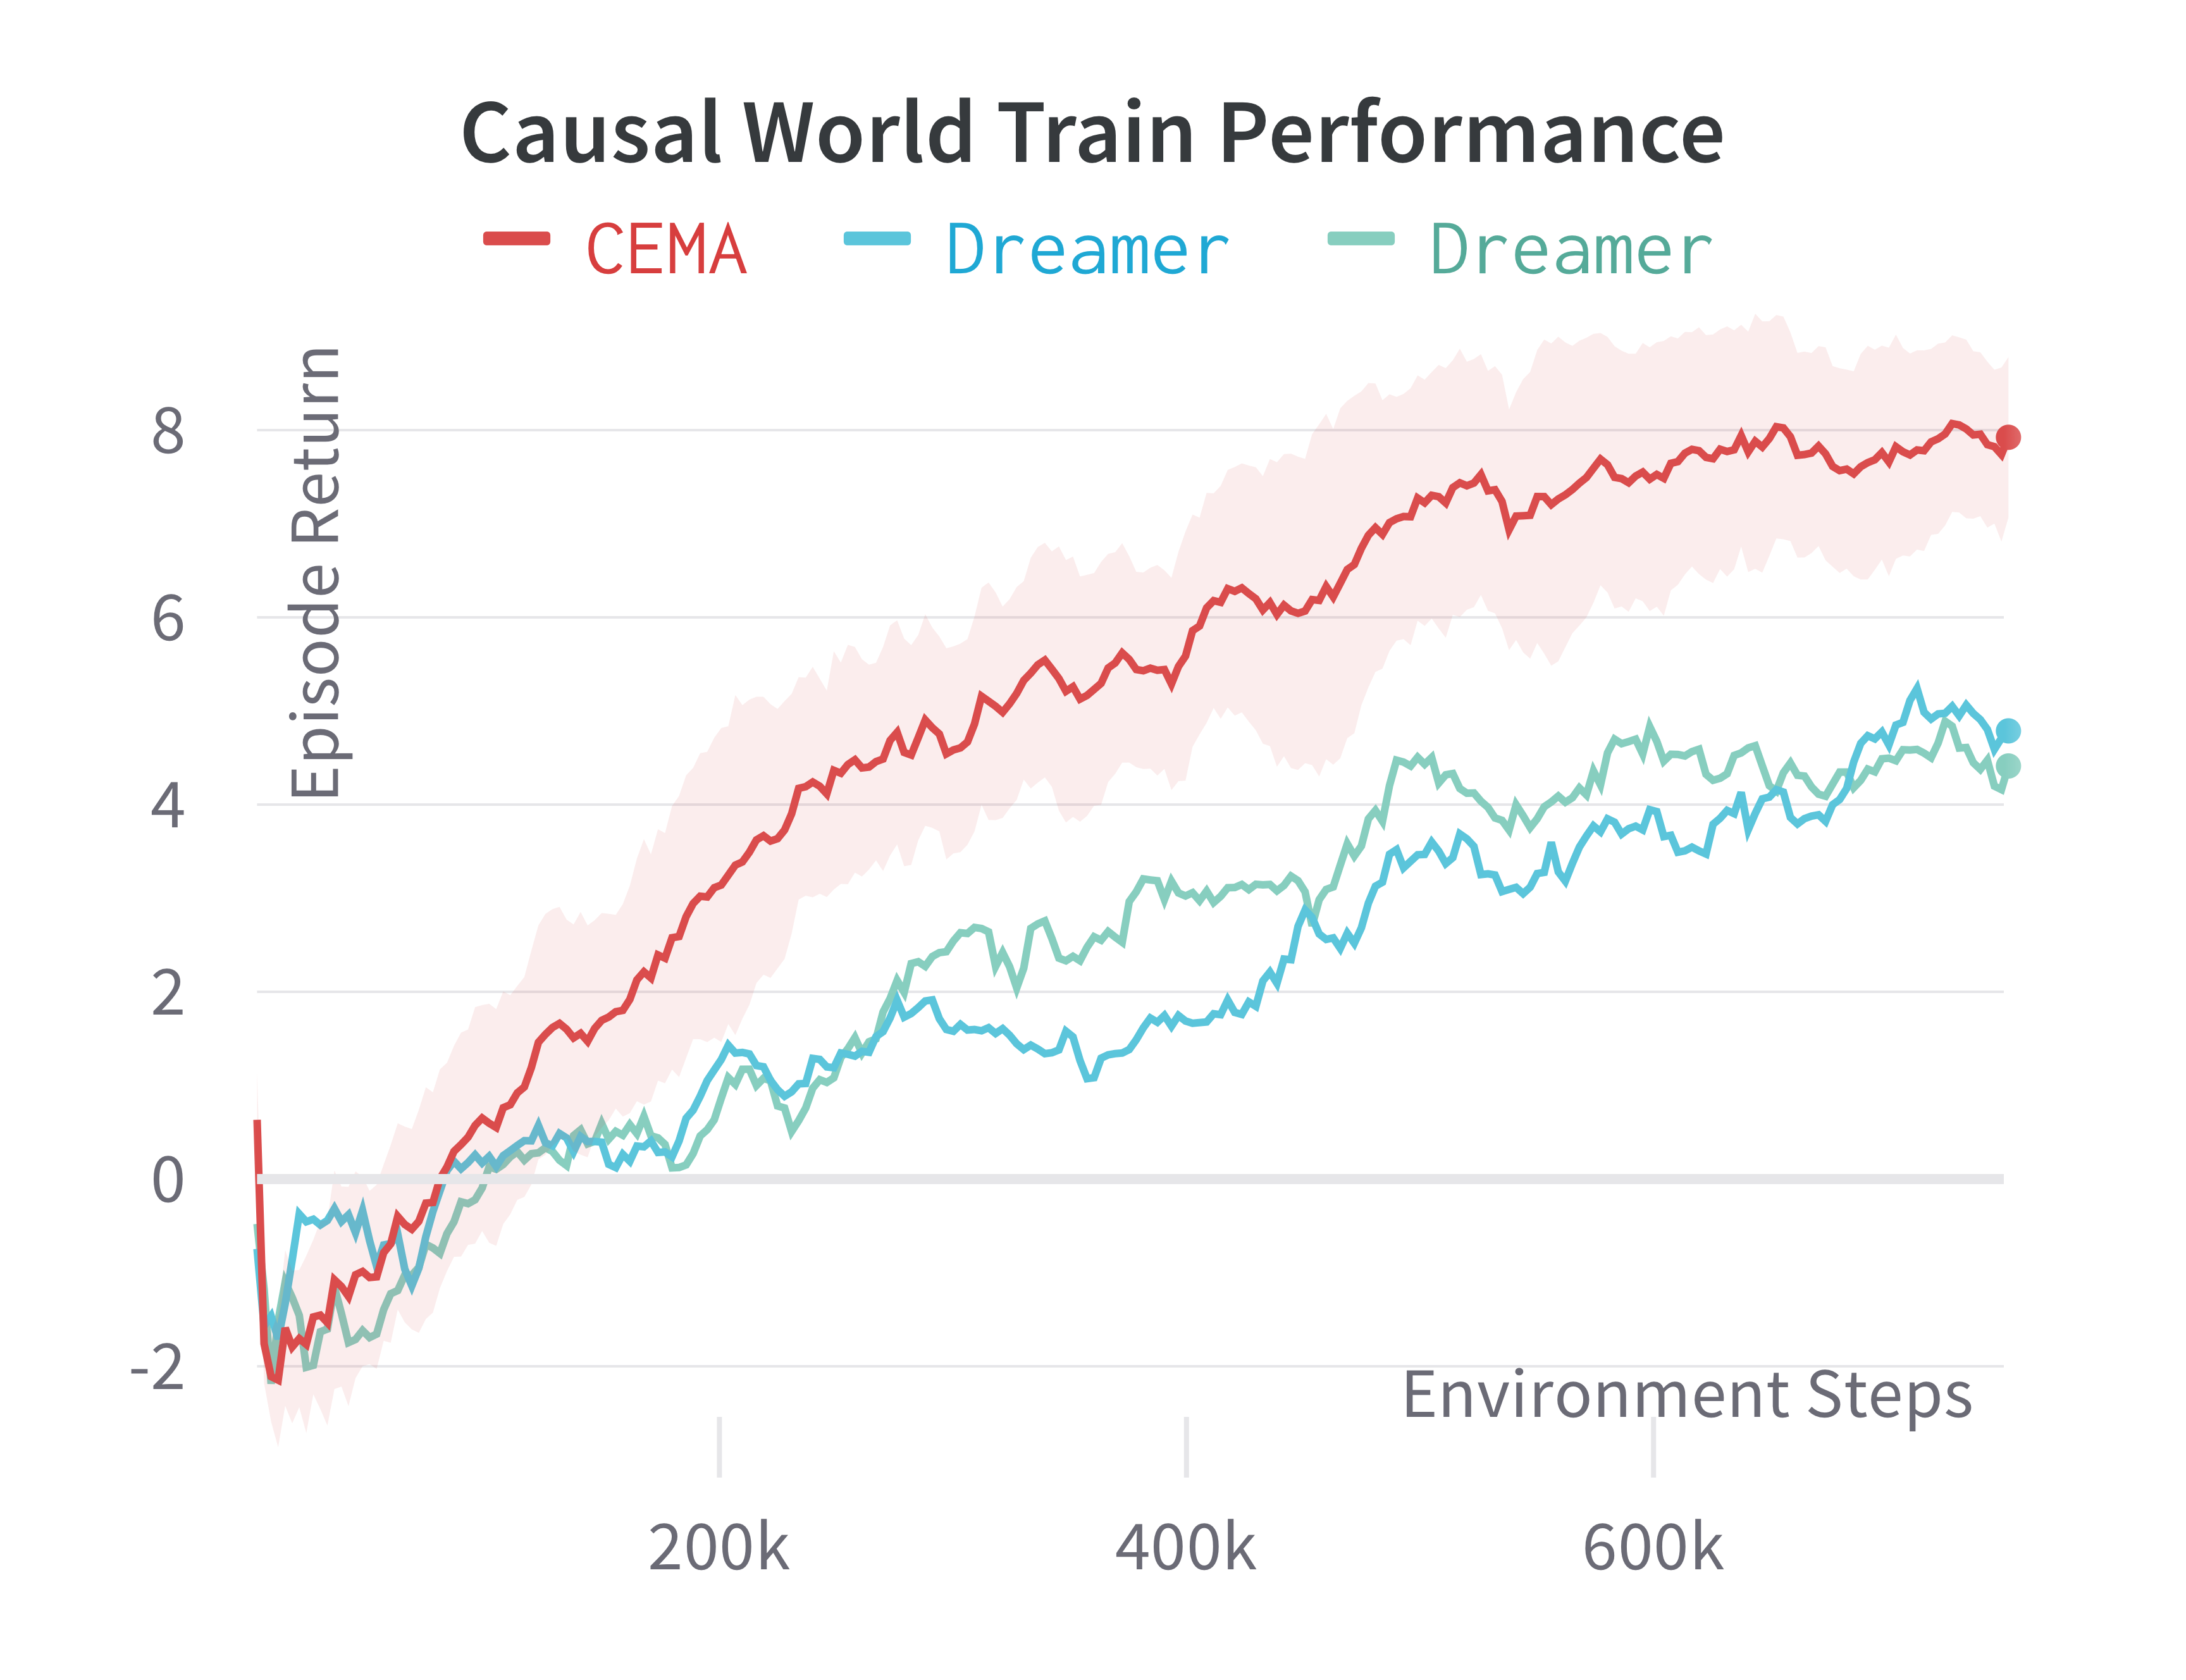
\includegraphics[height=0.5\paperheight]{images/performance/cema_res_cw.png}
        \end{subfigure}
      \caption{График наград на тренировочных задачах алгоритмов Dreamer и CEMA. Представленные награды являются неизмененными наградами среды.}
    \end{figure}
\end{column}
\note[item]<1->{The performance of CEMA on training tasks is slightly worse than Dreamer's in terms of task solving speed.}
\hfill
\begin{column}{0.48\linewidth}<2->
    \begin{figure}
        \begin{subfigure}{\linewidth}
          \centering
          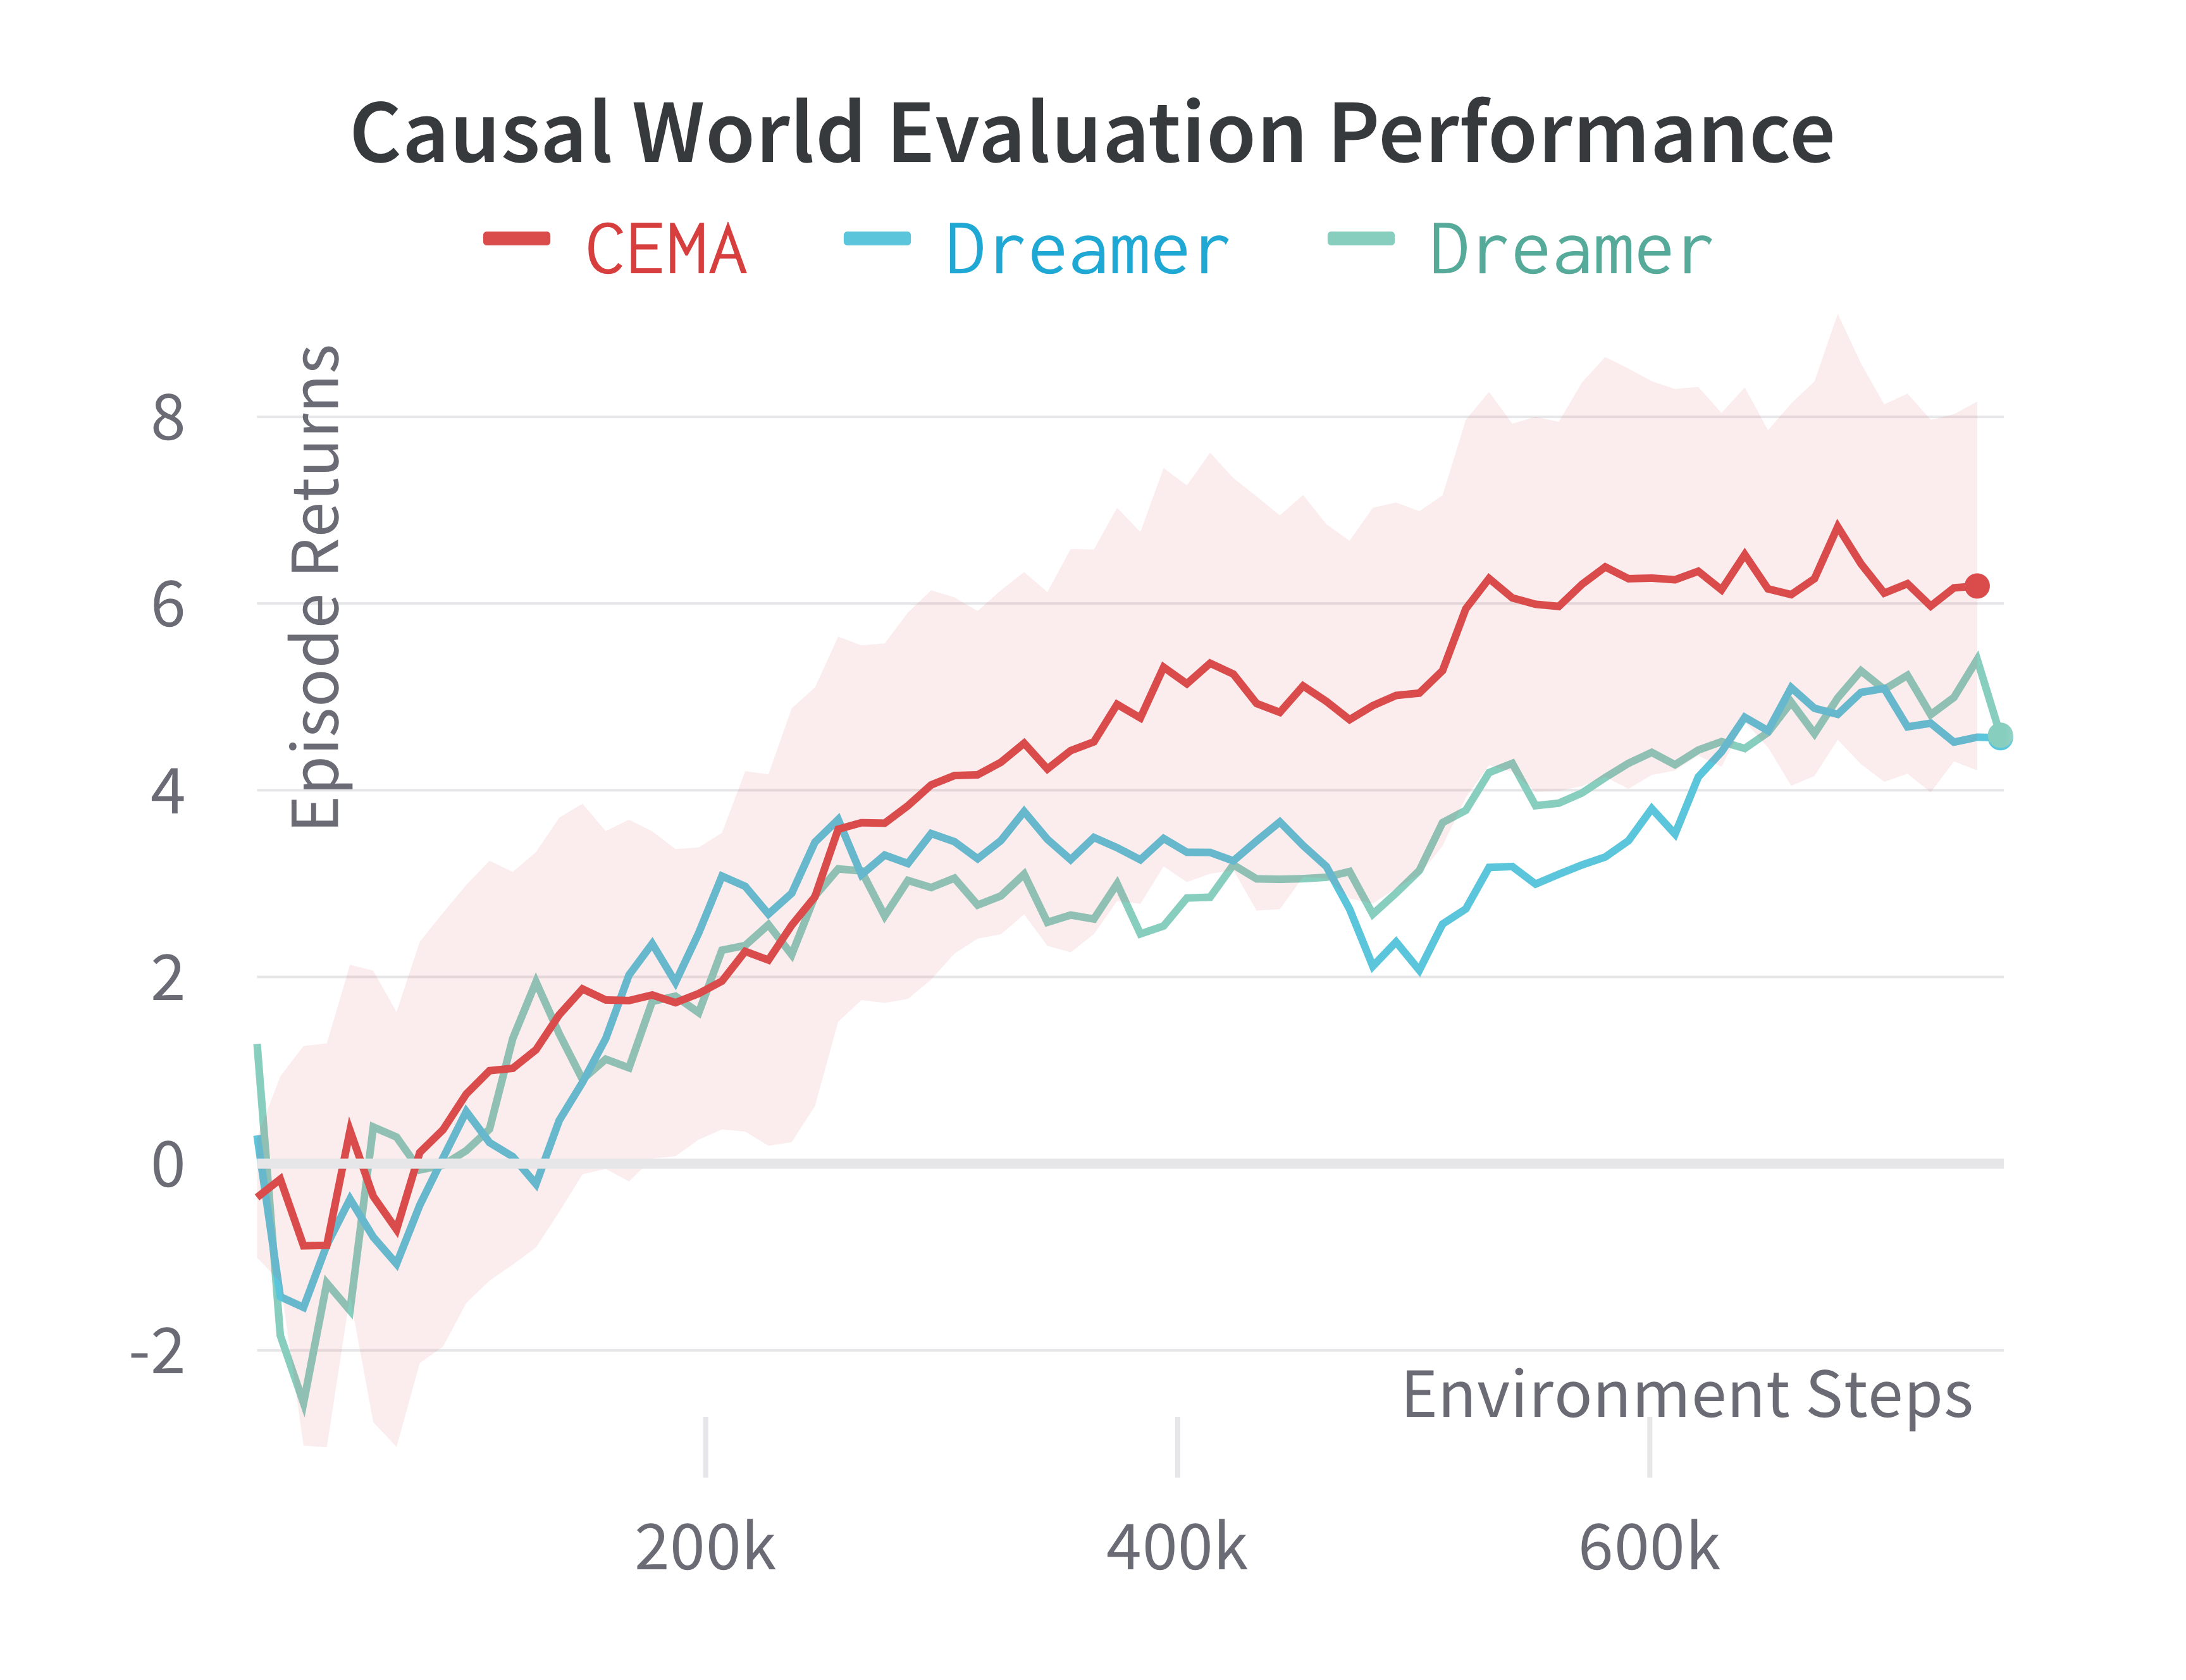
\includegraphics[height=0.5\paperheight]{images/performance/cema_eval_cw.png}
          \label{cw_gen_plot}
        \end{subfigure}
      \caption{Сравнение результатов работы алгоритма на тестовых задачах.}
    \end{figure}
\end{column}
\end{columns}
\note[item]<2->{However, its generalization capabilities are better - CEMA is able to solve more OOD tasks than Dreamer}
\end{frame}